\documentclass[11pt, oneside]{article}   	% use "amsart" instead of "article" for AMSLaTeX format
\usepackage{geometry}                		% See geometry.pdf to learn the layout options. There are lots.
\geometry{letterpaper}                   		% ... or a4paper or a5paper or ... 
%\geometry{landscape}                		% Activate for for rotated page geometry
%\usepackage[parfill]{parskip}    		% Activate to begin paragraphs with an empty line rather than an indent
\usepackage{graphicx}				% Use pdf, png, jpg, or eps� with pdflatex; use eps in DVI mode
								% TeX will automatically convert eps --> pdf in pdflatex		
\usepackage{amssymb}
\usepackage{amsmath}
\usepackage{hyperref}

\graphicspath{{/Users/telliott_admin/Dropbox/Tex/png/}}
\usepackage{parskip}

\title{A mole of popcorn}
%\author{The Author}
\date{}							% Activate to display a given date or no date

\begin{document}
\maketitle
%\section{}
%\subsection{}
\noindent
\large
In re-reading Walter Isaacson's biography of Einstein, I came across this about Avogadro's number:
\begin{center} 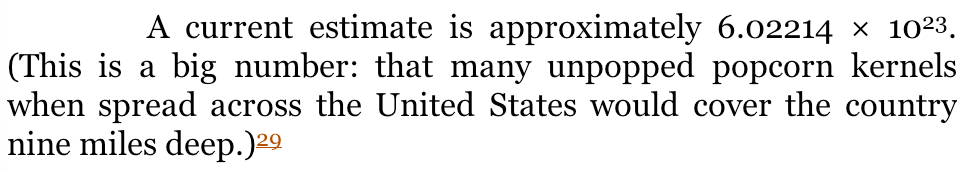
\includegraphics [scale=0.4] {popcorn-ref.png} \end{center}
Such an estimate is not particularly surprising, since  $10^{23}$ is a pretty big number.  "All the grains of sand on all the beaches in the world" is estimated to be $5 \times 10^{21}$.

\url{http://www.thenakedscientists.com/forum/index.php?topic=19016.0}

and a single grain of sand contains more atoms than that.  Anyway, let's check the estimate.  
\subsection*{Calculation}
According to wikipedia

\url{https://en.wikipedia.org/wiki/United_States}

the surface area of the the United States is $9,826,675 \text{ km}^2$, which is approximately $9.83 \times 10^{18} \text{ mm}^2$.  One mile is $1609$ meters or $1.61 \times 10^{6} \text{ mm}$, so the volume of the United States to a depth of one mile is about $1.58 \times 10^{25} \text{ mm}^3$.

If we take take the diameter of an (unpopped) popcorn kernel to be $4$ mm, then its volume is
\[ \frac{4}{3} \pi r^3 = \frac{4}{3} \times 3.14 \times 8 = 33.5 \text{ mm}^3 \]

\url{https://en.wikipedia.org/wiki/Sphere_packing}

Analysis of sphere packing suggests that the densest packing of small spheres in a volume where the boundaries are insignificant is about $74$\%, hence we require about $45.2$ mm$^3$ for each kernel.

Therefore, the number of kernels we can pack into that one-mile of depth is:
\[ \frac{1.58 \times 10^{25}}{45.2} \approx 3.5 \times 10^{23} \]

We seem to be a little short---more like a little bit under two miles.

If we consider just the \emph{land area}, then the volume in the numerator is reduced by a factor of 
\[ \frac{9.16}{9.83} \approx 0.93 \]

which helps some, but it still doesn't get us to $9$ miles.  More significant is our estimate of the volume of a kernel.  At our house we are big on popcorn (well, everyone but me), but it is this foo-foo stuff with really small kernels, which is not what I'm looking for here.

According to this

\url{https://answers.yahoo.com/question/index?qid=20090430104639AAc4XIv}

the diameter is more like $1/4$ inch or $6.5$ mm, giving a volume of $144$ mm$^3$, so with these corrections I obtain:

\[ \frac{1.58 \times 10^{25} \times 0.93}{144 / 0.74} \approx \frac{1.47 \times 10^{25}}{194} \approx 0.75 \times 10^{23} \]

which works out to a depth of 

\[ \frac{6.022}{0.75} \approx 8 \ \text{miles} \]

Close enough.
\end{document}  